\documentclass[a4paper,10pt]{article}
%\documentclass[a4paper,10pt]{scrartcl}

\usepackage[fleqn]{amsmath}
\usepackage{amsfonts}
\usepackage{amssymb}
\usepackage[utf8]{inputenc}
\usepackage{tabularx}
\usepackage{mathtools}
\usepackage{tikz}
\usepackage[hidelinks]{hyperref}
\usetikzlibrary{positioning}

\renewcommand{\tabularxcolumn}[1]{m{#1}}

\title{Discorn Protocol Motivation and Documentation}
\author{Suwako Moriya}
\date{2021}

\pdfinfo{%
  /Title    (Discorn Protocol Documentation)
  /Author   (SuwakoMmh)
  /Creator  (SuwakoMmh)
  /Producer (SuwakoMmh)
  /Subject  (Cryptography)
  /Keywords ()
}

\begin{document}
    \maketitle
    \tableofcontents
    \section{Why ?}
        Computers bring with them a new problem : It has become hard to get forgotten.
        Anything one shares with a company over the internet is potentially stored forever and used against them.
        Malicious entities such as hypothetical future governments might use such data against part of the population
        and endanger democracy.\\
        
        We defend a basic right to privacy and we are going to claim it no matter what thanks to cryptography.
        Bitcoin has opened the way with a trustless consensus protocol used in a currency. But the same idea
        can be used in many other applications. Discorn is a protocol that aims to achieve what apps such as Discord did,
        with the bonus of being open-source and decentralized.\\
        
        
        Examples of encrypted or decentralized messaging apps exists but we dislike the centralized nature of some of them
        and the federated nature of others. To put it simply:
        \begin{itemize}
         \item We dislike centralized software because it creates a single point of failure that governments can control
         if they please and because it relies on trust of a single third party.
        
         \item And we dislike federated software as well because it is a hassle to create a local instance : it requires web-related
         knowledge, a domain name, and the hardware to make it run. If one doesn't want to create a local instance because of all of that,
         then he has to trust a third party for his privacy. Which could be worse than the centralized alternative in some cases.
         We have been lead towards Matrix when our first ideas of Discorn emerged and yes, it does allow for chatting channels, VoIP and some kind of Guildish features.
         However we believe that we can do better both in usability and privacy.
        \end{itemize}
        The end-users, when using Discorn, not only helps claim a future for Humanity and get their privacy back. They also win the freedom
        of free software. Discorn can be modded, and nobody will be banned by Discorn. Because Discorn is no more than a protocol.
    
    \section{Structure}
        Discorn is organised around Chains. A Chain is a network of people sharing a Blockchain, it is created by one individual that claim its ownership. Being the owner of a Chain means having permission to promote
        new administrators, choosing who can join the network, which guild will be hosted, tweak other parameters.
        

    \section{Blockchain}
    
        \subsection{Block}
            To be valid, a block's hash must begin with a certain number of zeros. \\
            Let $X$ be the number of random hashes to mine a block with difficulty $d$, $X$ follows a geometric distribution : $Geo(\frac{1}{2^d})$. Hence : $\mathbb{E}(X)= 2^d$\\
            \begin{figure}[h]\centering
                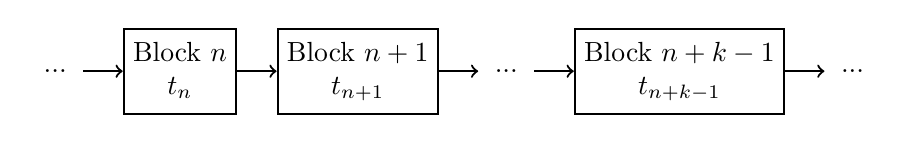
\begin{tikzpicture}[blocknode/.style={rectangle, draw=black, thick, minimum size=7mm},
                                    floatingnode/.style={rectangle, minimum size=7mm}, node distance=0.5cm]
                    \node[floatingnode] (0) {...};
                    \node[blocknode] (1) [right=of 0] {$\begin{matrix}\text{Block $n$}\\t_n\end{matrix}$};
                    \node[blocknode] (2) [right= of 1] {$\begin{matrix}\text{Block $n+1$}\\t_{n+1}\end{matrix}$};
                    \node[floatingnode] (3) [right= of 2] {...};
                    \node[blocknode] (4) [right= of 3] {$\begin{matrix}\text{Block $n+k-1$}\\t_{n+k-1}\end{matrix}$};
                    \node[floatingnode] (5) [right= of 4] {...};
                    \draw[thick,->] (0.east) -- (1.west);
                    \draw[thick,->] (1.east) -- (2.west);
                    \draw[thick,->] (2.east) -- (3.west);
                    \draw[thick,->] (3.east) -- (4.west);
                    \draw[thick,->] (4.east) -- (5.west);
                \end{tikzpicture}\caption{Blocks time interval.}\label{fig:Bti}
            \end{figure}\\
            
            Let $\Delta t$ be the average time interval between two blocks over a $k$ blocks interval.
            As seen in Fig \ref{fig:Bti}.
            \begin {align*}
             \Delta t = \frac{t_{n+k-1} - t_n}{k}
            \end {align*}

            
            To estimate the network's hashrate $N$ $[hash.s^{-1}]$, we use the following expression\\
            
            
            \begin {align*}
                &\text{}N = \frac{k\mathbb{E}(X)}{\Delta t} = \frac{k2^d}{\Delta t}\\
                &\text{We can express the next difficulty with ${\Delta t}_{target}$ and $k$}\\
                &N = \frac{k2^{d_{next}}}{{\Delta t}_{target}}\\
                &\Leftrightarrow 2^{d_{next}} = \frac{N{\Delta t}_{target}}{k}\\
                &\Leftrightarrow d_{next} = \left\lfloor\log_2\left(\frac{N{\Delta t}_{target}}{k}\right)\right\rfloor
            \end {align*}\\
            
            
            \noindent\begin{tabularx}{\textwidth}{|l|l|X|l|}
            \hline Field & Type & Description & Length \\ \hline
            \hline Version & big-endian int & Block version & 1 byte \\
            \hline Timestamp & big-endian int & & 4 bytes\\
            \hline Corner count & big-endian int & Number of Corner included & 3 bytes\\
            \hline Merkle root & cryptonight-fast-hash & Root hash of Corners Merkle tree & 32 bytes\\
            \hline Previous hash & cryptonight-slow-hash & Hash of previous block & 32 bytes\\
            \hline Difficulty & big-endian int & The calculated difficulty target being used for this block & 4 bytes\\
            \hline Nonce & raw & To allow variations of the header and compute different hashes & 4 bytes \\
            \hline
            \hline Corners & Corner list & Corners one after the other (Coinbase at index 0) & \\
            \hline
            \end{tabularx}
        
        
        \subsection{Corner}
            \begin{tabularx}{\textwidth}{|l|l|X|l|}
            \hline Field & Type & Description & Length \\ \hline
            \hline Payload length & big-endian int &  & 3 bytes \\
            \hline Payload flag ($P_{Flag}$) & big-endian int &  & 1 byte \\
            \hline Payload & raw & & \\
            \hline
            \end{tabularx}
            
            
            \subsubsection{Transaction (Tx):  $P_{Flag} = 0$}
                \begin{tabularx}{\textwidth}{|l|l|X|l|}
                \hline Field & Type & Description & Length \\ \hline
                \hline Version & big-endian int & Tx version & 1 byte \\
                \hline Input count & big-endian int & Number of Inputs included & 3 bytes\\
                \hline Input Puzzles & Input list & Transaction's inputs & \\
                \hline Output count & big-endian int & Number of Outputs included & 3 bytes\\
                \hline Output Puzzles & Puzzle list & Transaction's outputs & \\
                \hline Solutions & Solution list & To unlock each input, a Puzzle has to be solved. & \\
                \hline
                \end{tabularx}
            
            
            \subsubsection{Event: $P_{Flag} = 1$}
                \begin{tabularx}{\textwidth}{|l|l|X|l|}
                \hline Field & Type & Description & Length \\ \hline
                \hline Version & big-endian int & Event version & 1 byte \\
                \hline Hash & cryptonight-fast-hash & Event hash as in the event database & 32 Bytes\\
                \hline Authorization & Auth & Proof that the Event is legitimate & \\
                \hline
                \end{tabularx}\\
        
        
        \subsection{Input (Tx)}
            \begin{tabularx}{\textwidth}{|l|l|X|l|}
            \hline Field & Type & Description & Length \\ \hline
            \hline Hash & cryptonight-fast-hash & Input transaction's hash & 32 bytes \\
            \hline Index & big-endian int & Index of the specific output in the transaction & 3 byte \\
            \hline 
            \end{tabularx}

        \subsection{Output (Tx)}
            Amounts are coded on 12 bytes, unit is set at $10^{12}$ \\
            
            \begin{tabularx}{\textwidth}{|l|l|X|l|}
            \hline Field & Type & Description & Length \\ \hline
            \hline Amount & big-endian int & Amount sent & 12 bytes \\
            \hline Puzzle & Puzzle & Puzzle that protects the funds & \\
            \hline 
            \end{tabularx}

        \subsection{Puzzles \& Solutions (Tx)}
            \begin{tabularx}{\textwidth}{|l|l|X|l|}
            \hline Field & Type & Description & Length \\ \hline
            \hline Payload length & big-endian int &  & 3 bytes \\
            \hline Puzzle flag (${Pz}_{Flag}$) & big-endian int &  & 1 byte \\
            \hline Payload & raw & & \\
            \hline
            \end{tabularx}
            \subsubsection{Single: ${Pz}_{flag} = 0$}
                Simple, single address.
                \begin{itemize}
                 \item Puzzle:\\
                    
                    \begin{tabularx}{\textwidth}{|l|l|X|l|}
                        \hline Field & Type & Description & Length \\ \hline
                        \hline VK hash & cryptonight-fast-hash & Hash of the recipient public key. & 32 bytes \\
                        \hline
                    \end{tabularx}
                 \item Solution:\\
                 
                    \begin{tabularx}{\textwidth}{|l|l|X|l|}
                        \hline Field & Type & Description & Length \\ \hline
                        \hline Verifying key & VK &  & 64 bytes \\
                        \hline Tx Signature & Signature & Signature of the whole transaction without the Solutions part & 128 byte \\
                        \hline
                    \end{tabularx}
                \end{itemize}
        
        \subsection{Address}
            An address is a ``safe for human'' representation of a Puzzle.
            It is calculated as follows:
            
            $$\text{Address} = \text{base58}(\text{Puzzle + cryptonight-fast-hash}(\text{Puzzle})\text{[:4(bytes)]})$$

                
    \section{Event Database}
        \subsection{Event}
            Event structure is as follows:\\
            \begin{tabularx}{\textwidth}{|l|l|X|l|}
                \hline Field & Type & Description & Length \\ \hline
                \hline Version & big-endian int & Event version & 2 bytes \\
                \hline $P_{flag}$ & big-endian int & Payload identifier & 2 bytes \\
                \hline Payload & raw &  & \\
                \hline Veryfing key & VK & Key used for signing Payload & 64 bytes \\
                \hline Payload Signature & Signature & Signature of the Payload & 128 bytes \\
                \hline $A_{Flag}$ & big-endian int & & 2 bytes\\
                \hline Authority proof & Authority & & 2 bytes\\
                \hline
            \end{tabularx}
                \subsubsection{Message [Payload]: $P_{flag} = 0$}
                \subsubsection{Proof of Work [Authority]: $A_{flag} = 0$}
                    \begin{tabularx}{\textwidth}{|l|l|X|l|}
                        \hline Field & Type & Description & Length \\ \hline
                        \hline Target difficulty & big-endian int &  & 4 bytes \\
                        \hline Block hash & cryptonight-slow-hash & ($\sim$ Last) block hash & 32 bytes \\
                        \hline Block height & big-endian int & & 4 bytes \\
                        \hline Nonce & raw & & 32 bytes \\
                        \hline
                    \end{tabularx}
                \subsubsection{Nomination [Authority]: $A_{flag} = 1$}
                    \begin{tabularx}{\textwidth}{|l|l|X|l|}
                        \hline Field & Type & Description & Length \\ \hline
                        \hline Signing VK & VK &  & 64 bytes \\
                        \hline Signature & Signature & & \\
                        \hline
                    \end{tabularx}
    \section{Networking}
        \subsection{Sending data}
            Message structure is as follows :\\
            \begin{tabularx}{\textwidth}{|l|l|X|l|}
                \hline Field & Type & Description & Length \\ \hline
                \hline Version & big-endian int & Message version & 2 bytes \\
                \hline Payload flag & big-endian int & Payload identifier & 2 bytes \\
                \hline Payload & raw &  & \\
                \hline
            \end{tabularx}
            \subsubsection{IPV4}
                Connections are made over TCP.\\
                Messages are sliced in chunks of length CHUNK\_SIZE $=1024$.\\
                Chunks are sent one after the other over the TCP connection following this pattern:
                
                \noindent\begin{tabularx}{\textwidth}{|l|l|X|l|}
                    \hline Field & Type & Description & Length \\ \hline
                    \hline Length & big-endian int & 0xFFFF if not final, Chunk length otherwise & 2 bytes \\
                    \hline Data & raw & Chunk data & \\
                    \hline
                \end{tabularx}
        \subsection{Payloads}
        
            \subsubsection{Ping: $P_{Flag} = 1$}
                Send a ping request to remote.\\
                Expected behaviour: Send a pong message with the same id.\\
                
                \noindent\begin{tabularx}{\textwidth}{|l|l|X|l|}
                    \hline Field & Type & Description & Length \\ \hline
                    \hline Id & big-endian int & & 2 bytes \\
                    \hline
                \end{tabularx}
            
            \subsubsection{Pong: $P_{Flag} = 2$}
                Respond to a ping request from remote.\\
                Expected behaviour: None.\\
                
                \noindent\begin{tabularx}{\textwidth}{|l|l|X|l|}
                    \hline Field & Type & Description & Length \\ \hline
                    \hline Id & big-endian int & & 2 bytes \\
                    \hline
                \end{tabularx}
            
            \subsubsection{Heartbeat: $P_{Flag} = 3$}
                Notify remote that local is still up. (at a rythm of BPM times per minute.)\\
                Expected behaviour: Disconnect if no heartbeat was sent for $\frac{\text{TIMEOUT}}{\text{BPM}}$.\\
                
                \noindent\begin{tabularx}{\textwidth}{|l|l|X|l|}
                    \hline Field & Type & Description & Length \\ \hline
                \end{tabularx}
            
            \subsubsection{Getchain: $P_{Flag} = 4$}
                Initiate the Chain Challenge sequence.\\
                The Chain Challenge sequence is designed to allow
                peers to echange blockchain data safely,
                even in a MITM scenario.\\
                \begin{figure}[h]\centering
                    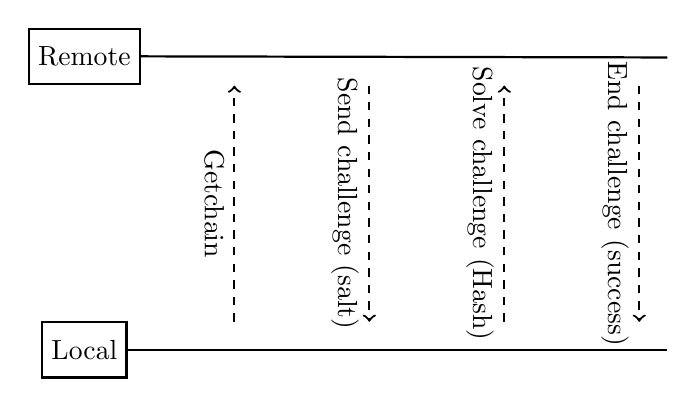
\begin{tikzpicture}[blocknode/.style={rectangle, draw=black, thick, minimum size=7mm},
                                    floatingnode/.style={rectangle, minimum size=7mm}, node distance=3cm and 1cm]
                    \node[blocknode] (0-0) {Remote};
                    \node[blocknode] (1-0) [below= of 0-0] {Local};
                    \node[floatingnode] (1-1) [right= of 1-0] {};
                    \node[floatingnode] (0-1) [above= of 1-1] {};
                    \node[floatingnode] (0-2) [right= of 0-1] {};
                    \node[floatingnode] (1-2) [below= of 0-2] {};
                    \node[floatingnode] (1-3) [right= of 1-2] {};
                    \node[floatingnode] (0-3) [above= of 1-3] {};
                    \node[floatingnode] (0-4) [right= of 0-3] {};
                    \node[floatingnode] (1-4) [below= of 0-4] {};
                    
                    \draw[thick,-] (0-0.east) -- (0-4.east) node[midway,sloped,anchor=north] {};
                    \draw[thick,-] (1-0.east) -- (1-4.east) node[midway,sloped,anchor=north] {};
                    \draw[thick, ->, dashed] (1-1.north) -- (0-1.south) node[midway,sloped,anchor=north, rotate=180] {Getchain};
                    \draw[thick, ->, dashed] (0-2.south) -- (1-2.north) node[midway,sloped,anchor=north] {Send challenge (salt)};
                    \draw[thick, ->, dashed] (1-3.north) -- (0-3.south) node[midway,sloped,anchor=north, rotate=180] {Solve challenge (Hash)};
                    \draw[thick, ->, dashed] (0-4.south) -- (1-4.north) node[midway,sloped,anchor=north] {End challenge (success)};
                    \end{tikzpicture}\caption{Chain Challenge sequence}\label{fig:GCSec}
                \end{figure}
                Expected behaviour: Send a Sendguildchallenge message.\\
                
                \noindent\begin{tabularx}{\textwidth}{|l|l|X|l|}
                    \hline Field & Type & Description & Length \\ \hline
                    \hline Id & big-endian int & & 2 bytes \\
                    \hline
                \end{tabularx}

            \subsubsection{Sendchainchallenge: $P_{Flag} = 5$}
                Send a salt for the Chain Challenge sequence.\\
                Expected behaviour: Send a Solvechainchallenge message with a hash of chain+salt\\
                
                \noindent\begin{tabularx}{\textwidth}{|l|l|X|l|}
                    \hline Field & Type & Description & Length \\ \hline
                    \hline Id & big-endian int & & 2 bytes \\
                    \hline Salt & raw & Random data & 16 bytes \\
                    \hline
                \end{tabularx}
            
            \subsubsection{Solvechainchallenge: $P_{Flag} = 6$}
                Send a hash of raw chain+salt from now on, the salted hash will be called RawChainChallenge\\
                Expected behaviour: Send an Endchainchallenge message\\
                
                \noindent\begin{tabularx}{\textwidth}{|l|l|X|l|}
                    \hline Field & Type & Description & Length \\ \hline
                    \hline Id & big-endian int & & 2 bytes \\
                    \hline Hash & cryptonight-fast-hash & rawchain+salt hash & 32 bytes \\
                    \hline
                \end{tabularx}
            
            \subsubsection{Endchainchallenge: $P_{Flag} = 7$}
                Notify successful or failed challenge.\\
                Expected behaviour : if successful, both Peers should now use the salted hash to reference the common Chain and every exchange about that chain should be AES encrypted with the raw chain hash (without salt) as a key.\\
                
                \noindent\begin{tabularx}{\textwidth}{|l|l|X|l|}
                    \hline Field & Type & Description & Length \\ \hline
                    \hline Id & big-endian int & & 2 bytes \\
                    \hline Success & big-endian int & 0 if successful & 1 byte \\
                    \hline
                \end{tabularx}
            
            \subsubsection{ChainData: $P_{Flag} = 8$}
                Send an encrypted chain message.\\
                Expected behaviour : Undefined.\\
                
                \noindent\begin{tabularx}{\textwidth}{|l|l|X|l|}
                    \hline Field & Type & Description & Length \\ \hline
                    \hline Chain & RawChainChallenge& & 32 bytes \\
                    \hline  & & Following data is AES encrypted & \\
                    \hline $CP_{Flag}$ & big-endian int & Payload identifier & 2 bytes \\
                    \hline Payload [Chain] & raw &  & \\
                    \hline 
                \end{tabularx}
            
            \subsubsection{Newhead [Chain]: $CP_{Flag} = 1$}
                Notify remote of a new chain head. (Doesn't send the block, just height and hash)\\
                Expected behaviour : None.\\
                
                \noindent\begin{tabularx}{\textwidth}{|l|l|X|l|}
                    \hline Field & Type & Description & Length \\ \hline
                    \hline Height & big-endian int & New head's height & 4 bytes \\
                    \hline Hash & cryptonight-slow-hash & New head's hash & 32 bytes\\
                    \hline
                \end{tabularx}

            \subsubsection{Getblockheader [Chain]: $CP_{Flag} = 2$}
                Ask remote for the block header at given height.\\
                Expected behaviour : Send a blockheader message.\\
                
                \noindent\begin{tabularx}{\textwidth}{|l|l|X|l|}
                    \hline Field & Type & Description & Length \\ \hline
                    \hline Height & big-endian int & New head's height & 4 bytes \\
                    \hline
                \end{tabularx}
            
            \subsubsection{Blockheader [Chain]: $CP_{Flag} = 3$}
                Sends a block header.\\
                Expected behaviour : None.\\
                
                \noindent\begin{tabularx}{\textwidth}{|l|l|X|l|}
                    \hline Field & Type & Description & Length \\ \hline
                    \hline Block header & Block header &  & 80 bytes \\
                    \hline
                \end{tabularx}

            \subsubsection{Getblockbody [Chain]: $CP_{Flag} = 4$}
                Ask remote for the block body at given height.\\
                Expected behaviour : Send a blockbody message.\\
                
                \noindent\begin{tabularx}{\textwidth}{|l|l|X|l|}
                    \hline Field & Type & Description & Length \\ \hline
                    \hline Height & big-endian int & New head's height & 4 bytes \\
                    \hline
                \end{tabularx}
            
            \subsubsection{Blockbody [Chain]: $CP_{Flag} = 5$}
                Sends a block body.\\
                Expected behaviour : None.\\
                
                \noindent\begin{tabularx}{\textwidth}{|l|l|X|l|}
                    \hline Field & Type & Description & Length \\ \hline
                    \hline Block height & big-endian int & & 4 bytes \\
                    \hline Block hash & cryptonight-slow-hash & & 32 bytes\\
                    \hline Block body & Block body& & \\
                    \hline
                \end{tabularx}
\end{document}
